\paragraph{QuizziPedia::Back-End::App::Models::SummaryModel}
\label{QuizziPedia::Back-End::App::Models::summaryModel}
\begin{figure}
	\centering
	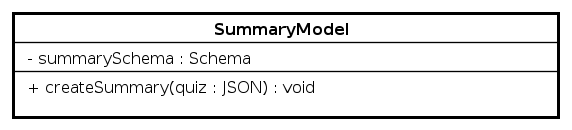
\includegraphics[scale=0.45]{UML/Classi/Back-End/QuizziPedia_Back-End_App_Models_summaryModel.png}
	\caption{QuizziPedia::Back-End::App::Models::summaryModel}
\end{figure}



\begin{itemize}
	\item \textbf{Descrizione} \\
	Classe che modella i riepiloghi all'interno dell'applicazione.
	\item \textbf{Utilizzo} \\
	Viene utilizzata per rappresentare i dati relativi ai riepiloghi all'interno dell'applicazione. Si interfaccia con la libreria \textit{Mongoose\ped{G}} per la creazione dello schema e dei relativi metodi statici o di istanza.
	\item \textbf{Relazioni con altre classi}
		............
	\item \textbf{Attributi}
		\begin{itemize}
			\item \textbf{- summarySchema: Schema} \\
			Questo campo dati rappresenta lo schema \textit{Mongoose\ped{G}} dei riepiloghi di \progetto. Lo schema prevede i seguenti attributi:
				\begin{itemize}
					\item \texttt{quiz} di tipo \texttt{ObjectId}, rappresenta il riferimento all'identificativo nel database del quiz;
					\item \texttt{givenAnswers} di tipo \texttt{Array}, contiene oggetti di tipo \texttt{ObjectId} che rappresentano i riferimenti agli identificativi nel database delle domande a cui si è risposto e due \texttt{Array} contenenti oggetti di tipo \texttt{String};	
					\item \texttt{date} di tipo \texttt{Date}, rappresenta la data di creazione del riepilogo;
					\item \texttt{mark} di tipo \texttt{Number}, rappresenta il voto conseguito nel quiz.
				\end{itemize}
		\end{itemize}
	\item \textbf{Metodi}
		\begin{itemize}
			\item \texttt{+ createSummary(quiz: JSON)}\\
			Crea un riepilogo.\\
			\textbf{Parametri}:
			\begin{itemize}
				\item \texttt{quiz: JSON}\\
				Rappresenta il quiz dalle cui risposte verrà creato il riepilogo.
			\end{itemize}
		\end{itemize}
\end{itemize}